\chapter{Registered Letters}
 
\ph[width = .99\textwidth]{../cape-of-good-hope/registered-letters/Registered_Cover.jpg}{ }

	 
 

Registration of letters appeared early in the Postal History of the 
Cape of Good Hope. Rhenius proclamation of the 2nd March 1792 provided 
for the establishment of a postal system at the Cape of Good Hope. 
This early postal system required that the Postmaster on payment of a 
fee of four stuivers, would record details of any letter or packet 
in a special book kept at the post office and would also make an 
annotation and append his signature above or below the seal which 
secured the letter or packet. No liability accrued to the post office, 
however in the event of a loss.

\ph[width = .99\textwidth]{../cape-of-good-hope/registered-letters/registered-01.jpg}{
Registered cover ex Worcester to Cape Town, franked pair 4d in almost sky blue shade, sitting hope tied by BONC 15 with "CAPE TOWN 22 DE 68" registered handstamp (Goldblatt Type RL 1). Worcester DTO backstamp on reverse.
}

\ph[width = .99\textwidth]{../cape-of-good-hope/registered-letters/registered-02.jpg}{
Registered cover ex Worcester to Cape Town, franked pair 4d on 6d overprint SG 27, tied by BONC 15 with "CAPE TOWN 1 MAR 69" registered handstamp (Goldblatt Type RL 1). Worcester DTO backstamp on reverse. Cover with original contents.
}

Establishment Of Registration Section in the Cape of Good Hope
With the spreading of post offices around the country a Registered 
Letter section was established at Cape Town's General Post Office 
to deal with this class of mail. By January 1854 the term 'Registered' 
was firmly established.
Registered Datestamps and handstamps in the Cape of Good Hope

\begin{marginfigure}
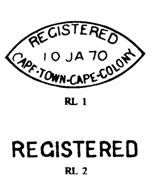
\includegraphics[width=1.0\textwidth]{../cape-of-good-hope/clip_image002_0000.jpg}
\end{marginfigure}

The first registered Letter datestamp  (RL1) was brought into 
use in the Cape of Good Hope shortly after 1854. It was, however, 
still necessary to write 'Registered' on the cover until about 1863-64, 
when a handstamp (RL2) replaced the manuscript marking.

On receipt of a registered letter the Postamaster would send an 
advice to the recipient to collect it.

\ph[width = .80\textwidth]{../cape-of-good-hope/registered-letters/early-receipt.jpg}{ }


The numbering of such letters was essential and the postmaster 
initially wrote the number on the envelope, alongside his office 
datestamp. Special registration handstamps (RL3 to 5) were 
introduced from 1909 onwards to facilitate the numbering.

  

A large variety of both circular and oval Registered Letter 
datestamps (RL 6 to 20) were in use. The horizontal oval 
handstamps (RL9 to RL18) were in most general use in colonial 
post offices for canceling adhesives whereas the circular ones 
were mostly used for back stamping of envelopes.
 
\ph[width = .60\textwidth]{../cape-of-good-hope/registered-letters/Receipt.jpg}{ }
 
Printed receipt forms, similar to those in use today, were available 
to senders a few years later.

 
\section{Registration Fees}

\ph[width = .90\textwidth]{../cape-of-good-hope/registered-letters/registered-triangular.jpg}{
1858 REGISTERED POST ENTIRE from Burghersdorp to Graaff Reinet franked 
pleasing colour combination of 6d deep rose-lilac (SG 7b) 
(paying 6d registration fee) and 4d deep blue (SG 6) (4d internal postage) 
triangulars, both tied by neat strikes of triangular defacer. 
Annotated "Regd" in manuscript. Rare, exceptionally attractive 
example of this rating. Photo-cert: PFSA. ..xnigk/111	
Price: \$ 2810
}

The registration fee was originally 6d. This was reduced to 4d in 1869 and to 
2 1/2 in 1897. Printed receipt forms similar to those in use today 
were available to senders of registered letters. 

\subsection{1855-65}

6d extra per letter

\subsection{1864}

On foreign letters sent by packet via the United Kingdom to Austria, Germany, Prussia, Saxony, Denmark, Norway, Sweden, united States and all British possessions: 1s. To Russia and Poland: 1s. 4d. if not exceeding a half ounce and 4d. for each additional half-ounce. To France and countries to which correspondence is forwarded through France: an additional amount equal to the amount of British or foreign postage.

\subsection{1869}

Inland including OFS, Transvaal and Natal 4d.

\subsection{1869-74}

Charge for registering to any part of the colony, neighbouring states 
or the United Kingdom: 4d per letter, book, sample packet or newspaper.

\subsection{1874-76}

Compulsory registered letters: Letters containing coin, 
as well as having the word 'Registered' written upon them, 
posted in the colony without registration, were registered 
and forwarded charged with a double registration fee.

\subsection{1897}

2 1/2 d per letter.

   
   
A number of Post Offices had their own straight line marks.   
\ph[width = .85\textwidth]{../cape-of-good-hope/AC289.jpg}{C289
1908 (December), KEVII 1d embossed postal stationery envelope sent registered to Cape Town, cancelled with a neat TYLDEN (28 Dec) single circle datestamp with a large handstruck ‘R’ in black alongside an unframed TYLDEN cachet in purple. The reverse with a further Tylden cds and a fine strike of the EASTERN / T.P.O. 4 (29.DEC.09 UP) double circle datestamp. A clean and attractive cover. (McGregor private lsiting) }   
   
   
                   